% diagrams/english/parque.tex -- el parque, para "Where is it?": el árbol
% grande (con una rama larga, para que se vea bien "on a branch"), el
% banco (con sitio debajo), el tobogán, el estanque con sus juncos y un
% arbusto. Se dibujan encima las cosas que dice el texto.
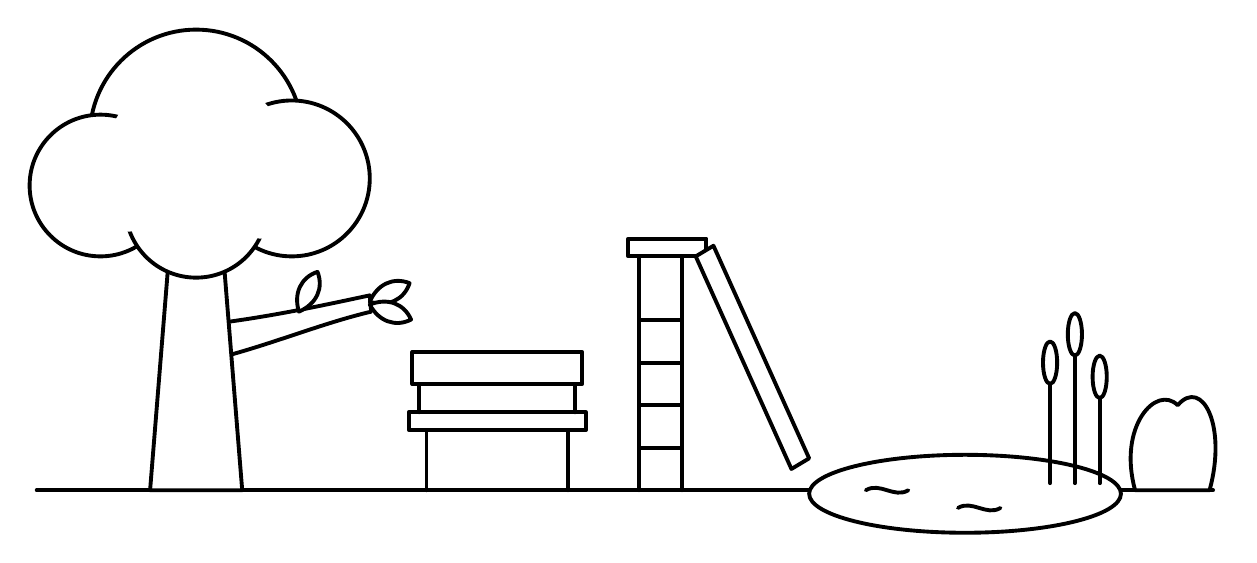
\begin{tikzpicture}[line width=1.4pt, line cap=round, line join=round, scale=0.9]
  % el suelo, cortado por el estanque
  \draw (-0.3,0) -- (10.6,0);
  \draw (15.0,0) -- (16.3,0);
  % la rama larga, que sale del tronco por debajo de la copa (se dibuja
  % antes, para que el tronco tape su arranque), con hojas en la punta
  \filldraw[fill=white] (2.2,2.35) .. controls (3.0,2.45) and (3.7,2.6) .. (4.4,2.75)
    -- (4.42,2.52) .. controls (3.7,2.35) and (3.0,2.05) .. (2.2,1.85) -- cycle;
  \foreach \x/\y/\a in {4.4/2.66/25, 4.4/2.62/-20, 3.4/2.52/65} {
    \filldraw[fill=white, shift={(\x,\y)}, rotate=\a]
      (0,0) .. controls (0.2,0.18) and (0.45,0.18) .. (0.62,0)
      .. controls (0.45,-0.18) and (0.2,-0.18) .. (0,0) -- cycle;
  }
  % el tronco y la copa
  \filldraw[fill=white] (1.3,0) -- (1.55,3.1) -- (2.35,3.1) -- (2.6,0) -- cycle;
  \filldraw[fill=white] (1.95,5.0) circle (1.5);
  \filldraw[fill=white] (0.6,4.3) circle (1.0);
  \filldraw[fill=white] (3.3,4.4) circle (1.1);
  \filldraw[fill=white] (1.95,4.0) circle (1.0);
  \fill[white] (1.95,4.6) circle (1.3);
  \fill[white] (2.9,4.45) circle (0.9);
  \fill[white] (1.0,4.4) circle (0.75);
  % el banco
  \draw (5.2,0) -- (5.2,0.85); \draw (7.2,0) -- (7.2,0.85);
  \filldraw[fill=white] (4.95,0.85) rectangle (7.45,1.1);
  \draw (5.1,1.1) -- (5.1,1.9); \draw (7.3,1.1) -- (7.3,1.9);
  \filldraw[fill=white] (5.0,1.5) rectangle (7.4,1.95);
  % el tobogán: la escalera, arriba la plataforma, y la rampa
  \draw (8.2,0) -- (8.2,3.3); \draw (8.8,0) -- (8.8,3.3);
  \foreach \y in {0.6,1.2,1.8,2.4} { \draw (8.2,\y) -- (8.8,\y); }
  \filldraw[fill=white] (8.05,3.3) rectangle (9.15,3.55);
  \filldraw[fill=white] (9.0,3.3) -- (10.35,0.3) -- (10.6,0.45) -- (9.25,3.45) -- cycle;
  % el estanque, con sus juncos a la derecha
  \filldraw[fill=white] (12.8,-0.05) ellipse (2.2 and 0.55);
  \draw (11.4,0.0) .. controls (11.6,0.12) and (11.8,-0.12) .. (12.0,0.0);
  \draw (12.7,-0.25) .. controls (12.9,-0.13) and (13.1,-0.37) .. (13.3,-0.25);
  \foreach \x/\h in {14.0/1.5, 14.35/1.9, 14.7/1.3} {
    \draw (\x,0.1) -- (\x,\h);
    \filldraw[fill=white] (\x,\h+0.3) ellipse (0.1 and 0.3);
  }
  % el arbusto
  \filldraw[fill=white] (15.2,0) .. controls (14.95,0.9) and (15.5,1.5) .. (15.8,1.2)
    .. controls (16.15,1.6) and (16.5,0.9) .. (16.25,0) -- cycle;
\end{tikzpicture}
